\RequirePackage{amsmath}
\RequirePackage{fix-cm}
\documentclass[deutsch]{svmono}

\def\ColoredLinks{}
%%%%%%%%%%%%%%%%%%%%%%%%%%%%%%%%%%%%%%%%%%%
% Alexanders Standardmacros - Version 3.0 %
%%%%%%%%%%%%%%%%%%%%%%%%%%%%%%%%%%%%%%%%%%%





%%%%%%%%%%%%%%%%%%%%%%%%%%%%%%%%%%%%%%%%%%%%%%%%
%  Farben für Links definieren                 %
%%%%%%%%%%%%%%%%%%%%%%%%%%%%%%%%%%%%%%%%%%%%%%%%

\ifdefined\ColoredLinks
  \def\linkColorLinkR{0}
  \def\linkColorLinkG{0}
  \def\linkColorLinkB{0.55}
	\def\linkColorCiteR{0}
  \def\linkColorCiteG{0}
  \def\linkColorCiteB{0.55}
	\def\linkColorUrlR{0}
  \def\linkColorUrlG{0}
  \def\linkColorUrlB{0.55}
\else
  \def\linkColorLinkR{0}
  \def\linkColorLinkG{0}
  \def\linkColorLinkB{0}
	\def\linkColorCiteR{0.3}
  \def\linkColorCiteG{0.3}
  \def\linkColorCiteB{0.3}
	\def\linkColorUrlR{0}
  \def\linkColorUrlG{0}
  \def\linkColorUrlB{0}
\fi





%%%%%%%%%%%%%%%%%%%%%%%%%%%%%%%%%%%%%%%%%%%%%%%%
%  Packages einbinden                          %
%%%%%%%%%%%%%%%%%%%%%%%%%%%%%%%%%%%%%%%%%%%%%%%%

%\usepackage{makeidx} - unterschägt manchmal Einträge
\usepackage{imakeidx} % Speziellen Features eigentlicht nicht verwendet, aber hat die makeidx-Fehler nicht
\usepackage[utf8]{inputenc}
\usepackage{amssymb}
\usepackage[ngerman]{babel}
\usepackage{epsf}
\usepackage[dvips]{rotating}
\usepackage{amsmath,amsfonts}
\usepackage[amsmath,thmmarks,noconfig]{ntheorem}
\usepackage{nameref}
\usepackage{hycolor}
\usepackage{hyperxmp}
\usepackage{hyperref}
\hypersetup{pdfauthor={Alexander Herzog},
            pdftitle={Warteschlangensimulator - Kurzeinführung},
            %pdfsubject={},
            %pdfkeywords={},
            pdfproducer={LaTeX},
            pdfcreator={pdfLaTeX},
						pdfcopyright={Copyright Alexander Herzog},
						pdfcontactcity={Clausthal-Zellerfeld},
						pdfcontactpostcode={38678},
						pdfcontactcountry={Deutschland},
						pdfcontactemail={alexander.herzog@tu-clausthal.de},
						pdfcontacturl={https://www.simzentrum.de,https://www.tu-clausthal.de},
						pdflang={de},
						bookmarksnumbered,
						colorlinks=true,
						filecolor=[rgb]{0,0,0},  % \href-Links nicht hervorheben
						linkcolor=[rgb]{\linkColorLinkR,\linkColorLinkG,\linkColorLinkB},
						citecolor=[rgb]{\linkColorCiteR,\linkColorCiteG,\linkColorCiteB},
						urlcolor=[rgb]{\linkColorUrlR,\linkColorUrlG,\linkColorUrlB} %\url{}, nur für E-Mail-Link genutzt
					}
\expandafter\def\expandafter\UrlBreaks\expandafter{\UrlBreaks
  \do\a\do\b\do\c\do\d\do\e\do\f\do\g\do\h\do\i\do\j
  \do\k\do\l\do\m\do\n\do\o\do\p\do\q\do\r\do\s\do\t
  \do\u\do\v\do\w\do\x\do\y\do\z\do\A\do\B\do\C\do\D
  \do\E\do\F\do\G\do\H\do\I\do\J\do\K\do\L\do\M\do\N
  \do\O\do\P\do\Q\do\R\do\S\do\T\do\U\do\V\do\W\do\X
  \do\Y\do\Z}
\usepackage{float}
\usepackage{fancyvrb}
\restylefloat{figure}
\restylefloat{table}
\usepackage{sectsty}
%\allsectionsfont{\fontfamily{cmss}\selectfont} - das führt zu Type 3 Fonts
\allsectionsfont{\sffamily\selectfont}
\usepackage{framed}
\usepackage[toc,page]{appendix}
\renewcommand\appendixname{Anhang}
\let\appendixtocname\appendixname\let\appendixpagename\appendixname
\usepackage[T1]{fontenc} % aus der pdf kopierbare Umlaute
\usepackage{eurosym}
\usepackage{longtable}

\usepackage{graphicx}
\usepackage[export]{adjustbox}




%%%%%%%%%%%%%%%%%%%%%%%%%%%%%%%%%%%%%%%%%%%%%%%%
%  Rotierte Tabellenüberschriften              %
%%%%%%%%%%%%%%%%%%%%%%%%%%%%%%%%%%%%%%%%%%%%%%%%

\usepackage{adjustbox}
\usepackage{array}
\usepackage{booktabs}
\usepackage{multirow}

\newcolumntype{R}[2]{%
    >{\adjustbox{angle=#1,lap=\width-(#2)}\bgroup}%
    l%
    <{\egroup}%
}
\newcommand*\rot{\multicolumn{1}{|R{90}{1em}|}}





%%%%%%%%%%%%%%%%%%%%%%%%%%%%%%%%%%%%%%%%%%%%%%%%
%  Symbole definieren                          %
%%%%%%%%%%%%%%%%%%%%%%%%%%%%%%%%%%%%%%%%%%%%%%%%

\newcommand{\setH}{\mathbb{H}}
\newcommand{\setC}{\mathbb{C}}
\newcommand{\setR}{\mathbb{R}}
\newcommand{\setQ}{\mathbb{Q}}
\newcommand{\setZ}{\mathbb{Z}}
\newcommand{\setN}{\mathbb{N}}
\newcommand{\comp}{\complement}
\newcommand{\Umg}{{\cal U}}

\newcommand{\calA}{{\cal A}}
\newcommand{\calB}{{\cal B}}
\newcommand{\calC}{{\cal C}}
\newcommand{\calD}{{\cal D}}
\newcommand{\calE}{{\cal E}}
\newcommand{\calF}{{\cal F}}
\newcommand{\calG}{{\cal G}}
\newcommand{\calH}{{\cal H}}
\newcommand{\calI}{{\cal I}}
\newcommand{\calJ}{{\cal J}}
\newcommand{\calK}{{\cal K}}
\newcommand{\calL}{{\cal L}}
\newcommand{\calM}{{\cal M}}
\newcommand{\calN}{{\cal N}}
\newcommand{\calO}{{\cal O}}
\newcommand{\calP}{{\cal P}}
\newcommand{\calQ}{{\cal Q}}
\newcommand{\calR}{{\cal R}}
\newcommand{\calS}{{\cal S}}
\newcommand{\calT}{{\cal T}}
\newcommand{\calU}{{\cal U}}
\newcommand{\calV}{{\cal V}}
\newcommand{\calW}{{\cal W}}
\newcommand{\calX}{{\cal X}}
\newcommand{\calY}{{\cal Y}}
\newcommand{\calZ}{{\cal Z}}

\def\arccot{\mathop{\rm arccot}}
\def\Arcoth{\mathop{\rm Arcoth}}
\def\Arsinh{\mathop{\rm Arsinh}}
\def\Artanh{\mathop{\rm Artanh}}
\def\Arcosh{\mathop{\rm Arcosh}}

\def\d{{\rm d}}
\def\dx{\d x}
\def\dy{\d y}
\def\dz{\d z}
\def\dt{\d t}
\def\euler{\mathrm{e}}

\def\id{{\rm id}}
\def\Kern{{\rm Kern}}

\def\ra{\Rightarrow}

\def\oversym#1#2{\mathop{#1}\limits^{#2}}
\def\Inneres#1{\oversym{#1}\circ}


\def\TO#1{\oversym\longrightarrow{#1}}
\def\RA#1{\oversym\Longrightarrow{#1}}
\def\IFF#1{\oversym\iff{#1}}
\def\gleich#1{\oversym={#1}}

\def\oBdA{o.\,B.\,d.\,A.\ }

\renewcommand{\qed}{\begin{flushright} $\square$ \end{flushright}}

\def\Definition#1{{\bf #1}}

\def\E{{\bf E}}
\def\Var{{\bf Var}}
\def\Std{{\bf Std}}
\def\CV{{\bf CV}}
\def\SCV{{\bf SCV}}





%%%%%%%%%%%%%%%%%%%%%%%%%%%%%%%%%%%%%%%%%%%%%%%%
%  Umgebungen definieren                       %
%%%%%%%%%%%%%%%%%%%%%%%%%%%%%%%%%%%%%%%%%%%%%%%%

%\theoremstyle{changebreak}
%\theoremheaderfont{\normalfont\bfseries}
%\theoremseparator{:}
%\theoremsymbol{}
%\newtheorem{definition}{Definition}[chapter]
%\newtheorem{satz}[definition]{Satz}
%\newtheorem{hilfssatz}[definition]{Hilfssatz}
%\newtheorem{lemma}[definition]{Lemma}
%\newtheorem{beispiel}[definition]{Beispiel}
%\newtheorem{beispiele}[definition]{Beispiele}
%\newtheorem{bezeichnung}[definition]{Bezeichnung}
%\theorembodyfont{\rmfamily}
%\newtheorem{bemerkung}[definition]{Bemerkung}
%\newtheorem{vereinbarung}[definition]{Vereinbarung}
%\newtheorem{folgerung}[definition]{Folgerung}
%\theoremheaderfont{\normalfont\bfseries}
%\theoremstyle{nonumberchangebreak}
%\theorembodyfont{\rmfamily}
%\theoremsymbol{$\blacksquare$}
%\newtheorem{beweis}{Beweis}
%\theoremsymbol{}





%%%%%%%%%%%%%%%%%%%%%%%%%%%%%%%%%%%%%%%%%%%%%%%%
%  Standard epsilon durch schöneres ersetzen   %
%%%%%%%%%%%%%%%%%%%%%%%%%%%%%%%%%%%%%%%%%%%%%%%%

\def\epsilon{\varepsilon}





%%%%%%%%%%%%%%%%%%%%%%%%%%%%%%%%%%%%%%%%%%%%%%%%
%  Verbatim-Umgebungen für verschiedene Zwecke %
%%%%%%%%%%%%%%%%%%%%%%%%%%%%%%%%%%%%%%%%%%%%%%%%

\DefineVerbatimEnvironment{ExcelVerbatim}{Verbatim}{frame=single,label=Excel-Befehl,fontsize=\small}
\DefineVerbatimEnvironment{ExcelVerbatimWithMath}{Verbatim}{frame=single,label=Excel-Befehl,commandchars=\\\{\},codes={\catcode`$=3\catcode`^=7},fontsize=\small}
\DefineVerbatimEnvironment{ExcelVerbatimWithFormat}{Verbatim}{frame=single,label=Excel-Befehl,fontsize=\small,commandchars=\\\{\}}
\DefineVerbatimEnvironment{RVerbatim}{Verbatim}{frame=single,label=R-Code,fontsize=\small}
\DefineVerbatimEnvironment{ExcelMacroVerbatim}{Verbatim}{frame=single,label=Excel-Makro,fontsize=\small} % ,numbers=left
\DefineVerbatimEnvironment{ExcelMarcroVerbatimWithMath}{Verbatim}{frame=single,label=Excel-Makro,commandchars=\\\{\},codes={\catcode`$=3\catcode`^=7},fontsize=\small}
\DefineVerbatimEnvironment{ExcelMacroVerbatimWithFormat}{Verbatim}{frame=single,label=Excel-Makro,fontsize=\small,commandchars=\\\{\}}
\newcommand{\sub}[2]{{#1_#2}}

\newcommand{\newlinesymbol}{\rotatebox[origin=c]{270}{$\curvearrowright$}}





%%%%%%%%%%%%%%%%%%%%%%%%%%%%%%%%%%%%%%%%%%%%%%%%
%  Formatierungen                              %
%%%%%%%%%%%%%%%%%%%%%%%%%%%%%%%%%%%%%%%%%%%%%%%%

%\def\emphasis#1{\textbf{#1}}
%\def\emphasisBFOnly#1{\textbf{#1}}
\def\emphasis#1{\emph{#1}}
\def\emphasisBFOnly#1{#1}

\def\emphasisIT#1{\textit{#1}}
\def\emphasisEnglish#1{\textit{#1}}

%\font\deutschfont=suet14
%\def\deutsch#1{\hbox{\deutschfont #1}}

\parindent0pt
\parskip5pt

%\oddsidemargin4.6mm
%\evensidemargin-5.4mm
%\textwidth160mm
\usepackage{xcolor}
\usepackage{lmodern}
\usepackage{wrapfig}
\textwidth160mm
\textheight220mm
\oddsidemargin0mm
\evensidemargin0mm
\topmargin0mm

\def\cmd#1{\textbf{,,\texttt{#1}''}}
\def\cm#1{\textbf{\texttt{#1}}}

\begin{document}

\thispagestyle{empty}
\vskip5cm {\Huge\textbf{Kurzeinführung \vskip.1cm Warteschlangensimulator}}
\vskip.5cm \hrule
\vskip.5cm {\large \textsc{Alexander Herzog} (\href{mailto:alexander.herzog@tu-clausthal.de}{alexander.herzog@tu-clausthal.de})}
\IfFileExists{../../Warteschlangennetz-mittel.png}{
\vskip2cm \centerline{\fbox{\includegraphics[width=16cm]{../../Warteschlangennetz-mittel.jpg}}}
}{}
\vskip2cm {\color{gray}
Dieses Tutorial bezieht sich auf die Version 4.6.0
 des Warteschlangensimulators.\\
Download-Adresse: \href{https://a-herzog.github.io/Warteschlangensimulator/}{https://a-herzog.github.io/Warteschlangensimulator/}.
}
\renewcommand{\thepage}{\roman{page}}

{
\clearpage
\pdfbookmark{Inhaltsverzeichnis}{Inhaltsverzeichnis}
\begingroup \let\cleardoublepage\relax \tableofcontents \endgroup
}



\chapter{Einleitung}

\renewcommand{\thepage}{\arabic{page}}
\setcounter{page}{1}

Der Warteschlangensimulator ist ein Programm zur ereignisorientierten stochastischen Simulation von Warteschlangenmodellen. In dem Programm können Produktions- und Logistikprozesse, die stochastischen Einflüssen (Schwankungen im Kundenankunftsstrom, variable Bedienzeiten, ...) und auch deterministischen Einflüssen (zeitabhängige Verfügbarkeit von Ressourcen, ...) unterliegen, abgebildet und simuliert werden.

Der Warteschlangensimulator verfügt über einen schnellen, mehrkernfähigen und (für ein Java-Programm) speichereffizienten Simulationskern, der auch in der Lage ist, große Modelle zu simulieren. Da der Simulator durchgängig auf das offene XML-Dateiformat setzt, lassen sich solche großen Modelle auch sinnvoll importieren. Allerdings besteht das Hauptanwendungsfeld des Programms darin, Modelle interaktiv in dem Programm in Form von Fließbildern zu entwerfen. Da die grafische Darstellung eines Modells ab einer gewissen Größe anfängt, unübersichtlich zu werden, sind eher kleine bis mittlere Modelle das primäre Einsatzgebiet des Simulators. Aufgrund der verhältnismäßig kurzen Simulationslaufzeiten können schnell Was-wäre-wenn Untersuchungen durchgeführt werden und verschiedene Steuerungsalternativen verglichen werden. Unterstützt wird dieses Konzept durch Funktionen wie die automatische Parameterreihen Erstellung: Nach der Vorgabe eines Modells und eines zu variierenden Parameters, wird das entsprechende Modell für jeden vorgewählten Wert simuliert und die Ergebnisse werden in nutzerdefinierter Form als Tabelle ausgegeben. Auf diese Weise kann die Auswirkung der Änderung eines Parameters sehr einfach untersucht werden.



\chapter{Programmoberfläche}

\begin{figure}[h]	
	\caption{Programmfenster des Warteschlangensimulators}
	\centerline{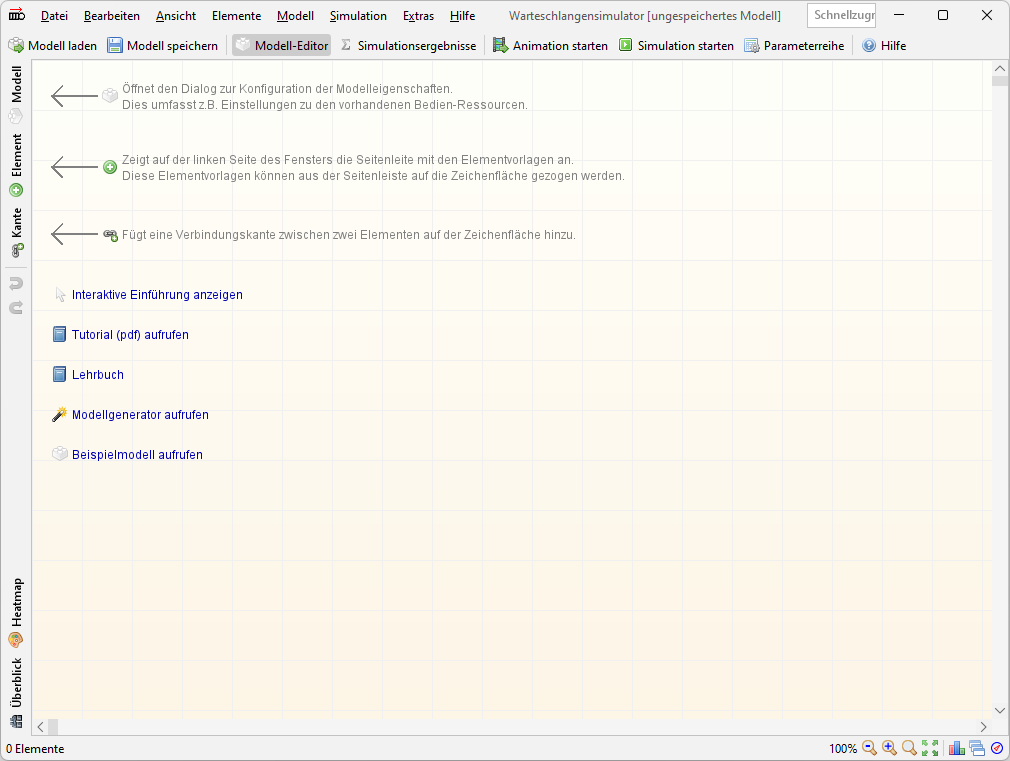
\includegraphics[width=14cm]{ProgramWindow.png}}
	\label{fig:ProgramWindow}
\end{figure}
 
Nach dem Programmstart ist direkt die Zeichenfläche, auf der die Fließbilder angelegt werden können, zu sehen.

In der oberen Symbolleiste gibt es die beiden Schaltflächen \textbf{Modell-Editor} und \textbf{Simulationsergebnisse}, mit denen zwischen den beiden Hauptprogrammfunktionen umgeschaltet werden kann:

\begin{itemize}
\item
Der \textbf{Modell-Editor} stellt die Zeichenfläche, auf der das Simulationsmodell als Fließbild modelliert werden kann, dar. Zusätzlich werden über die linke Symbolleiste Werkzeuge zur Bearbeitung des Modells angezeigt.
\item
Die \textbf{Simulationsergebnis}-Ansicht wird nach dem Abschluss eines Simulationslaufs automatisch aktiviert und stellt die Ergebnisse in Form von Texten, Tabellen und Grafiken dar. Neben der Möglichkeit zum Export dieser einzelnen Dokumente können über die Simulationsergebnis-Ansicht auch Reports erstellt werden und die Ergebnisse in nutzerdefinierter Form gefiltert werden.
\end{itemize}



\chapter{Der Modell-Editor}

Der Modell-Editor besteht im Wesentlichen aus einer großen Zeichenfläche, die fast die gesamte Fläche des Programmfensters einnimmt. Zusätzlich existiert am linken Fensterrand eine vertikale Symbolleiste, über die Elemente und Verbindungskanten in das Simulationsfließbild eingefügt werden können und generelle Einstellungen zu dem Modell vorgenommen werden können.

\section{Vertikale Symbolleiste}

Die drei wesentlichen Schaltflächen in der vertikalen Symbolleiste sind:

\begin{itemize}
\item
\textbf{Modell:}\\
Über diese Schaltfläche lässt sich ein Dialog öffnen, in dem diverse Einstellungen zu dem Simulationsmodell vorgenommen werden können (Simulationslaufzeit, verfügbare Ressourcen, Eigenschaften der simulierten Kunden usw.).
\item
\textbf{Element:}\\
Durch das Anklicken dieser Schaltfläche lässt sich die Elementen-Vorlagen-Leiste am linken Fensterrand ein- und ausklappen. Aus dieser Vorlagenleiste können die Elemente per Drag\&Drop auf die Zeichenfläche gezogen werden.
\item
\textbf{Kante:}\\
Ein Simulationsfließbild besteht aus zwei Arten von Objekten: Elementen (auch Stationen genannt), an denen Aktionen stattfinden, und Verbindungskanten zwischen den Stationen. Die Elemente können aus der ausgeklappten Elementen-Vorlagen-Leiste per Drag\&Drop an beliebige Stellen auf die Zeichenfläche gezogen werden und später auch beliebig verschoben werden. Hierbei gibt es zunächst keine Einschränkungen: Elemente können sich theoretisch überlappen -– was jedoch später das Modell unübersichtlich machen würde -– oder beliebig weit voneinander entfernt sein. Kanten hingegen können nicht eigenständig existieren. Eine Kante verbindet stets zwei Elemente. Kanten werden als Pfeile dargestellt, d.\,h.\ es ist auch stets ein Richtung von einem Ausgangs- zu einem Zielelement vorgegeben. Da Kanten immer mit Elementen in Verbindung stehen müssen, können diese nicht einfach aus der Vorlagenleiste auf die Zeichenfläche gezogen werden, sondern es müssen stets Start- und Zielelement einer Kante definiert werden. Wird die Kante-Schaltfläche angeklickt, so bleibt diese farbig hinterlegt, bis sie erneut angeklickt wird, um die Funktion wieder zu deaktivieren. So lange die Kante-Funktion aktiviert ist, können Kanten durch das nacheinander Anklicken von Start- und Zielelement in das Modell eingefügt werden. Ob das Element, auf das jeweils mit der Maus gezeigt wird, als Ausgangs- oder Zielelement in Frage kommt, wird durch die jeweilige Form des Mauszeigers signalisiert.
\end{itemize}

\section{Zeichenfläche}

Aus der Vorlagenleiste auf die Zeichenfläche gezogene Elemente können mit gedrückter linker Maustaste verschoben werden.

Sollen mehrere Elemente gleichzeitig verschoben werden, so können diese nacheinander mit gedrückter Umschalt-Taste angeklickt werden oder es kann mit gedrückter linker Maustaste ein Rahmen um sie gezogen werden, um so mehrere Elemente zu selektieren.

Über das Kontextmenü oder durch Drücken der Entfernen-Taste können die selektierten Elemente gelöscht werden.
Ebenfalls über das Kontextmenü oder per Doppelklick oder per Druck der Tastenkombination Strg+Enter kann zu allen Elementen ein Bearbeiten-Dialog geöffnet werden, in dem die Eigenschaften des jeweiligen Elements eingestellt werden können.

Statt per Maus können die selektierten Elemente auch über die Cursortasten verschoben werden: Wird die Alt-Taste gedrückt gehalten, so können die jeweils selektierten Elemente mit den Cursortasten auf der Zeichenfläche verschoben werden. Die Elemente werden dabei an einem Raster ausgerichtet. Wird zusätzlich die Umschalt-Taste gedrückt gehalten, so können die Elemente vollkommen frei pixelgenau verschoben werden.



\chapter{Vorstellung eines einfachen Warteschlangenmodells}

Das einfachste mögliche Warteschlangenmodell besteht aus drei Elementen:

\begin{itemize}
\item
eine Quelle,
\item
einer Bedienstation und
\item
einem Ausgang.
\end{itemize}

Diese drei Elemente können aus der Vorlagenleiste auf der linken Fensterseite auf die Zeichenfläche gezogen werden (ggf. dafür zunächst auf die Element-Schaltfläche klicken, um die Seitenleiste einzublenden). Danach können die Elemente über die Kante-Schaltfläche verknüpft werden: Klicken Sie dafür zunächst auf ,,Kante'', um das Einfügen von Kanten zu aktivieren. Klicken Sie dann nacheinander auf die Kundenquelle und dann auf die Bedienstation, um die erste Kante einzufügen, und dann auf Bedienstation und danach auf den Kundenausgang auf der Zeichenfläche, um die zweite Kante einzufügen.
 
\begin{figure}[H]	
	\caption{Einfaches Warteschlangenmodell im Modell-Editor}
	\centerline{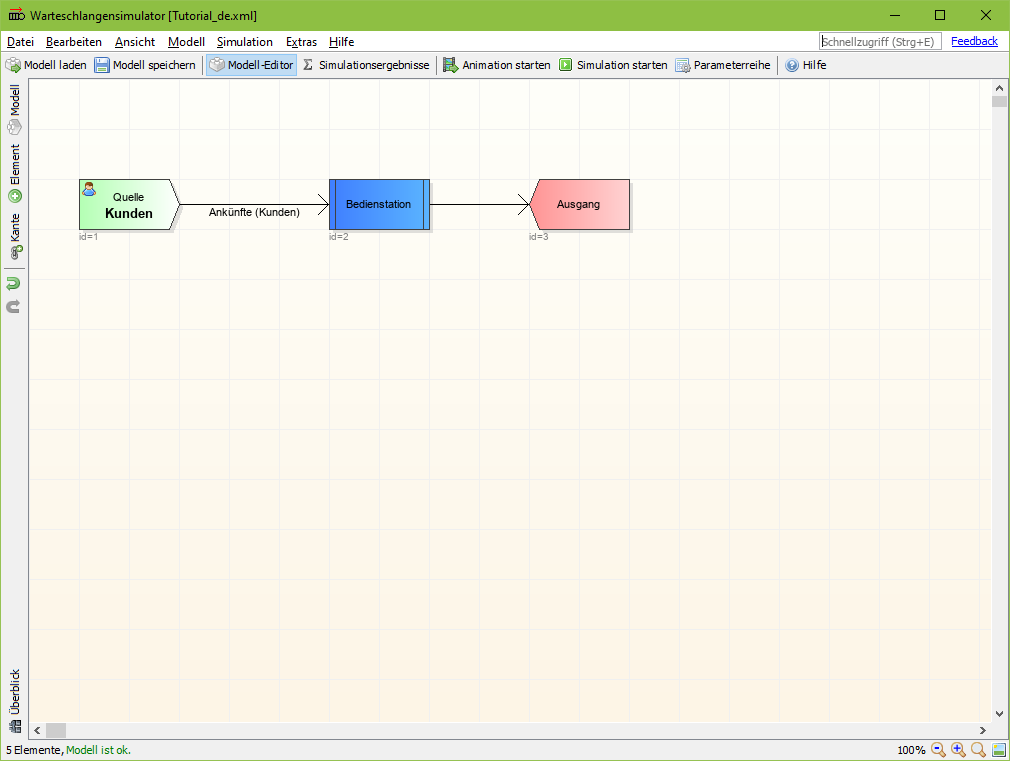
\includegraphics[width=14cm]{ProgramWindowModel.png}}
	\label{fig:ProgramWindowModel}
\end{figure}

Der Weg der Kunden durch das System beginnt stets an einer Quelle und endet stets an einem Ausgang. Während der Ausgang über keine weiteren Konfigurationsmöglichkeiten verfügt, müssen die Kundenquelle und die Bedienstation im Folgenden konfiguriert werden, um das Modell simulieren zu können.

\section{Konfiguration der Kundenquelle}

\begin{wrapfigure}{l}{2.25cm}
\vspace{-22pt}
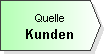
\includegraphics[width=2cm]{IconSource.png}
\vspace{-22pt}
\end{wrapfigure}
Per Doppelklick auf das Kundenquelle-Element lässt sich der Einstellungen-Dialog für dieses Element öffnen.

\begin{figure}[H]	
	\caption{Dialog ,,Quelle bearbeiten''}
	\centerline{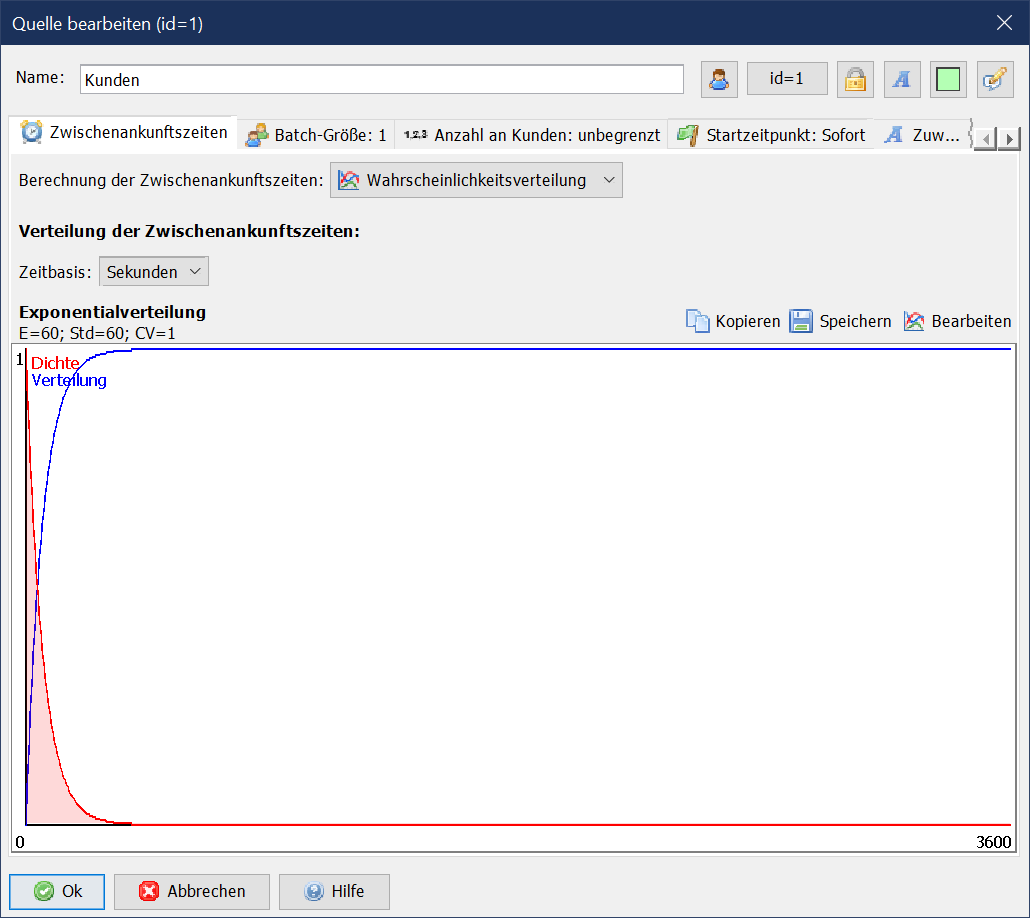
\includegraphics[width=10cm]{DialogSource.png}}
	\label{fig:DialogSource}
\end{figure}
 
In dem Name-Feld kann der Kundentyp der in dieser Quelle zu generierenden Kunden eingestellt werden. Die Kenngrößen der an dieser Station generierten Kunden werden unter diesem Namen später in der Statistik ausgewiesen. Die Kundenquelle generiert, sofern nicht anders eingestellt, bis zum Ende der Simulation fortwährend weitere Kunden und leitet diese über die Ausgangskante aus dem Element zum nächsten Element weiter (im Falle dieses einfachen Beispiels zur Bedienstation).

Die Zeitpunkte der Kundenankünfte werden dabei über die Zwischenankunftszeiten, d.\,h.\ die Zeitdauern zwischen der Ankunft von zwei aufeinander folgenden Kunden, definiert. Die Festlegung der Zwischenankunftszeiten kann in dem Kundenquelle-Element auf verschiedene Arten erfolgen: Über eine Wahrscheinlichkeitsverteilung, über einen Ausdruck, dessen Wert nach jeder Kundenankunft neu berechnet wird und in den der aktuelle Systemzustand einfließen kann, über einen Zeitplan, über eine Bedingung, die erfüllt sein muss, damit ein neuer Kunde eintreffen darf, oder über ein oder mehrere Signale, die eine Kundenankunft auslösen. Für das aktuelle Beispiel soll die Bestimmung der Zwischenankunftszeiten über eine Wahrscheinlichkeitsverteilung beibehalten werden, d.\,h.\ der Vorgabewert des \textbf{Berechnung der Zwischenankunftszeiten} Feldes kann beibehalten werden. Unter diesem Feld werden im Falle der Verwendung einer Wahrscheinlichkeitsverteilung die Dichte und die Verteilungsfunktion dargestellt. Über die \textbf{Bearbeiten}-Schaltfläche kann der Verteilungseditor geöffnet werden, in dem die Verteilung konfiguriert wird. Für dieses Modell kann als Zwischenankunftszeitenverteilung die Exponentialverteilung mit einem Erwartungswert, d.\,h.\ mit einem mittleren Abstand zwischen zwei Kundenankünften, von 60 Sekunden beibehalten werden.

Über die weiteren Dialogelemente in dem ,,Quelle bearbeiten''-Dialog kann eingestellt werden, ob die Kunden jeweils einzeln (Vorgabeeinstellung) oder in Gruppen eintreffen sollen. Außerdem kann angegeben werden, dass die Kundenquelle nur eine begrenzte Anzahl an Kunden generieren soll. Für dieses erste Modell können die Einstellungen in diesen Bereichen unverändert übernommen werden.

\section{Konfiguration der Bedienstation}

\begin{wrapfigure}{l}{2.25cm}
\vspace{-22pt}
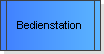
\includegraphics[width=2cm]{IconProcess.png}
\vspace{-22pt}
\end{wrapfigure}
Die Bedienstation ist in den meisten Warteschlangenmodellen das zentrale Element. Auch hier lässt sich per Doppelklick auf das Bedienstation-Element ein Einstellungen-Dialog öffnen.

\begin{figure}[H]	
	\caption{Dialog ,,Bedienstation bearbeiten''}
	\centerline{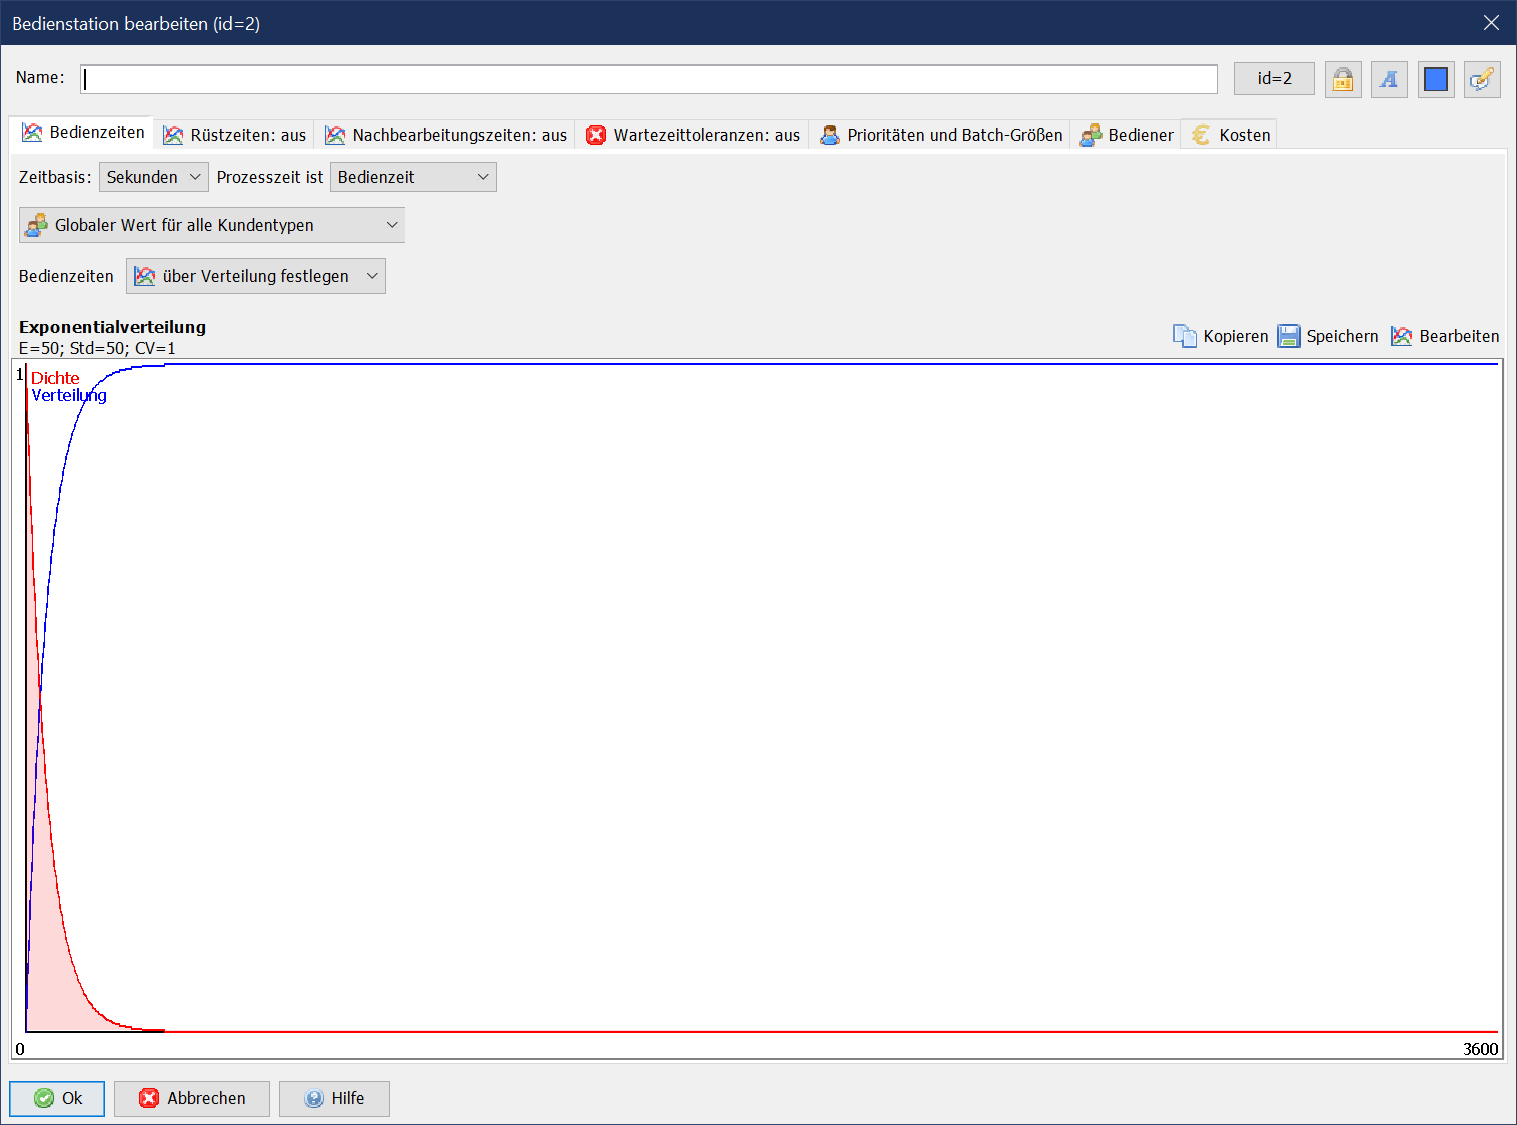
\includegraphics[width=14cm]{DialogProcess.png}}
	\label{fig:DialogProcess}
\end{figure}
 
Der Name der Bedienstation hat keine Funktion für die Simulation. Wichtiger sind hier die Einstellungen, die über die unter dem Name-Feld befindlichen Registerreiter vorgenommen werden können.

\begin{itemize}
\item
\textbf{Bedienzeiten:}\\
Auf dieser Dialogseite kann eingestellt werden, wie lange die Bedienungen der Kunden dauern sollen. Die Bedienzeiten können dabei über eine Verteilungsfunktion oder über einen Ausdruck, dessen Wert bei jeder Bedienung neu berechnet wird und in den der aktuelle Systemzustand einfließen kann, definiert werden. Bei der Verwendung einer Verteilungsfunktion stehen auch hier alle üblichen Wahrscheinlichkeitsverteilungen zur Verfügung (wieder bearbeitbar über die ,,Bearbeiten''-Schaltfläche). Da auch eine Ein-Punkt-Verteilung vorhanden ist, können auch deterministische Bedienzeiten vorgegeben werden. Über das Auswahlfeld ,,\textbf{Prozesszeit ist ...}'' kann eingestellt werden, ob die Bedienzeit an dieser Station für die Kunden als Bedienzeit, als Transferzeit oder optional auch als Wartezeit für die Statistik gezählt werden soll. Auf diese Weise lassen sich z.\,B.\ Transferzeiten zwischen den Stationen abbilden: Zwischen den eigentlichen Bedienstationen können Pseudo-Bedienstationen angelegt werden, deren Bedienzeiten als Transferzeiten verbucht werden.
Bei der Definition der Bedienzeiten ist es wichtig darauf zu achten, dass die Bediener im Mittel in der Lage sind, die eintreffenden Kunden bedienen zu können. In dem aktuellen Beispiel wurde eine mittlere Zwischenankunftszeit von 60 Sekunden gewählt. Als Vorgabewert beträgt die mittlere Bediendauer 50 Sekunden, was bedeutet, dass der Bediener im Mittel schnell genug ist, um die eintreffenden Kunden bedienen zu können.
\item
\textbf{Rüstzeiten:}\\
Auf dieser Dialogseite können zusätzliche Zeiten, die zwischen der Bedienung gleich oder - was meist der Fall ist - Kunden verschiedener Typen auftreten definiert werden. Diese für jeden Kundentyp-Übergang optionalen Rüstzeiten können jeweils entweder über eine Wahrscheinlichkeitsverteilung oder einen Ausdruck definiert werden.
\item
\textbf{Nachbearbeitungszeiten:}\\
Nach jeder Bedienung eines Kunden kann sich für den Bediener eine sogenannte Nachbearbeitungsphase anschließen, bevor er wieder für die Bedienung des nächsten Kunden verfügbar ist. Der Kunde befindet sich während der Nachbearbeitungszeit bereits nicht mehr in der Bedienstation, d.\,h.\ für ihn hat die Nachbearbeitungszeit keine Bedeutung. Allerdings verringert sich durch die Nachbearbeitungszeiten die verfügbare Bedienleistung: Benötigt ein Bediener pro Kunde im Mittel 60 Sekunden Bedienzeit und 30 Sekunden Nachbearbeitungszeit, so kann er im Mittel nicht 60 Kunden pro Stunde bedienen, sondern nur noch 40. In diesem ersten Beispiel sollen keine Nachbearbeitungszeiten verwendet werden.
\item
\textbf{Wartezeittoleranzen:}\\
Evtl. verfügen die eintreffenden Kunden nur über eine begrenzte Wartebereitschaft. Sofern es sich bei den ,,Kunden'' um Werkstücke in einem Produktionsprozess handelt – und diese Werkstücke nicht verderblich sind – kann von einer unbegrenzten Wartezeittoleranz ausgegangen werden. Bei menschlichen Kunden oder der Verarbeitung von verderblichen Waren muss jedoch unterstellt werden, dass diese nur begrenzt lange bereit sind zu warten. Auf der Dialogseite ,,Wartezeittoleranzen'' kann eingestellt werden, gemäß welcher Wahrscheinlichkeitsverteilung bzw. gemäß welchen Ausdrucks die Wartezeittoleranzen der Kunden bestimmt werden sollen. Verwendet eine Bedienstation Wartezeittoleranzen, so muss das Element über zwei Ausgänge verfügen: Einen für die erfolgreich bedienten Kunden und einen für die Warteabbrecher. In diesem ersten Beispiel soll auf die Modellierung von Wartezeittoleranzen verzichtet werden.
\item
\textbf{Prioritäten und Batch-Größen:}\\
Treffen an einer Bedienstation Kunden mehrerer Typen ein, so kann es gewollt sein, diese unterschiedlich zu priorisieren, d.\,h.\ einzelne Kundengruppen bevorzugt zu bedienen. Auf dieser Dialogseite kann für jede Kundengruppe eine Formel angegeben werden, gemäß derer ihre Priorität bestimmt wird. Die Variable ,,w'' steht dabei für die bisherige Wartezeit des Kunden. Wird ,,w'' als Formel verwendet, so erfolgt die Bedienung nach dem First-come-first-serve Prinzip: Der Kunde, der bereits am längsten wartet, wird als nächstes Bedient.
Des Weiteren kann eingestellt werden, dass die Kunden nicht einzeln, sondern in Gruppen (in sogenannten Batches) bedient werden. Ist eine Batch-Größe von 2 eingestellt, so muss ein einzelner in einer leeren Bedienstation neu eingetroffener Kunde warten, bis ein zweiter Kunde eingetroffen ist. Die Bedienzeit der beiden Kunden zusammen entspricht dann der auf der ersten Dialogseite angegebenen Bedienzeit, d.\,h.\ die beiden Kunden werden gleichzeitig und nicht nacheinander bedient. In diesem Beispiel sollen die First-come-first-serve Bedienung, d.\,h.\ ,,w'' als Priorität für die Kunden, sowie eine Batch-Größe von 1, d.\,h.\ die individuelle Bedienung der Kunden, beibehalten werden.
\item
\textbf{Bediener:}\\
Das wichtigste Element einer Bedienstation sind die Bediener. In Bezug auf die Bediener sind diverse Kombinationen abbildbar – die alle über die Möglichkeiten analytischer Warteschlangenmodelle hinausgehen: Es können mehrere Bediener notwendig sein, um eine Bedienung durchzuführen und gleichzeitig können mehrere Bediener verfügbar sein. Die Bediener werden dabei in mehrere Gruppen untergliedert. Die notwendige und die verfügbare Anzahl an Bedienern können dabei pro Gruppe variieren. Des Weiteren können mehrere verschiedene Bedienstationen dieselben Bedienergruppen nutzen. So können in einem Kantinen-Modell z.\,B.\ die Stationen ,,Essensausgabe A'', ,,Essensausgabe B'' und ,,Essensausgabe C'' jeweils die Ressource ,,Bediener A'', ,,Bediener B'' oder ,,Bediener C'' benötigen (von denen jeweils eine Person zur Verfügung steht), aber zusätzlich noch die Ressource ,,Suppenkelle'' benötigen, von der insgesamt für alle Stationen zusammen nur zwei zur Verfügung stehen. Noch einen Schritt weiter können auch vollständig verschiedene Alternativen, wie ein Kunde bedient werden kann, definiert werden. D.\,h.\ es können sowohl Und-Verknüpfungen definiert werden (,,Es müssen die Ressourcen A und B verfügbar sein.'') als auch Oder-Verknüpfungen (,,Ein Kunde kann durch Bediener A oder Bediener B bedient werden.'') definiert werden und beide Varianten kombiniert werden.

Über die \textbf{Ressourcen-Priorität} kann eingestellt werden, mit welcher Priorität bestimmte Stationen bei gleichzeitigen Anfragen auf eine Ressource durch mehrere Stationen Zugriff auf die Ressource erhalten sollen. Je höher die Priorität ist, desto höher ist die Wahrscheinlichkeit, dass eine Station die Ressource erhält. Die Ressourcen werden dabei nur dann reserviert, wenn alle notwendigen Ressourcen gleichzeitig verfügbar sind. Auf diese Weise werden Dead-Lock-Situationen vermieden. (So kann es nicht passieren, dass ,,Essensausgabe A'' die ,,Suppenkelle'' bereits reserviert hat und ,,Essensausgabe B'' den ,,Bratenspieß'', aber zur Bedienung eines Kunden an einer der Stationen beides notwendig ist und sich so beide Stationen gegenseitig blockieren.)

Zur Bedienung eines Kunden muss mindestens eine Bedienergruppe in der Bedienstation eingetragen werden. Die Bedienergruppen können über den Modelleigenschaften-Dialog im Detail konfiguriert werden. Allerdings können neue Bedienergruppen auch direkt über den Bedienstation-Dialog angelegt werden. Klicken Sie auf die ,,\textbf{Notwendige Bedienergruppe hinzufügen}''. Es öffnet sich ein Dialog, in dem eingestellt werden kann, ob eine bereits existente Bedienergruppe an dieser Station eingesetzt werden soll oder ob eine neue Bedienergruppe angelegt werden soll. Da es bisher noch keine Bedienergruppen in dem System gibt, wird nur die Option zum Anlegen einer neuen Gruppe angeboten. Neue Gruppen bestehen zunächst stets aus einem Bediener (änderbar über den Modelleigenschaften-Dialog). In dem vorliegenden Beispiel beträgt die mittlere Zwischenankunftszeit 60 Sekunden und die mittlere Bediendauer 50 Sekunden, d.\,h.\ eine Gruppe aus einem Bediener ist ausreichend, um die eintreffenden Kunden bedienen zu können. In dem Dialog zum Hinzufügen einer Bedienergruppe kann optional noch ein Name für die neue Bedienergruppe angegeben werden (unter diesem Namen wird die Auslastung der Bediener später in der Statistik ausgewiesen).
\item
\textbf{Kosten:}\\
Auf der Kosten-Seite des Bedienstation-Bearbeiten-Dialogs kann eingestellt werden, welche Kosten durch die Bedienung eines Kunden (bzw. einer Kundengruppe im Falle der Batch-Bearbeitung) pauschal oder/und pro Bedien- und pro Nachbearbeitungssekunde anfallen. Bei diesen Kosten handelt es sich um die Kosten aus Sicht der Bedienstation selbst. Kosten auf Kundenseite (Kosten pro Warte-, Transfer- und Bediensekunde) sowie Kosten für die Bediener (Kosten pro Verfügbarkeitsstunde, pro gearbeiteter Stunde und pro Leerlaufstunde) können jeweils in dem Modelleigenschaften-Dialog eingestellt werden. Kosten können grundsätzlich auch negativ sein; auf diese Weise können Gewinne abgebildet werden. Über das Element ,,Kosten'' können an beliebiger Stelle im Fließbild auch Kosten oder Gewinne (z.\,B.\ wenn ein Kunde das System erfolgreich bedient verlässt) direkt abgebildet werden.
\end{itemize}



\chapter{Simulation und Statistikausgabe}

Damit sollte dieses erste Modell bereits vollständig einsatzbereit sein. Falls Sie kein Modell anlegen wollen, aber dennoch die nächsten Schritte ausprobieren wollen, so können Sie auch über den Menüpunkt Datei|Beispiel laden|Erlang-C-Vergleichsmodell ein Modell in den Editor laden, welches abgesehen von etwas anderen Zwischenankunfts- und Bedienzeiten mit dem oben beschriebenen Modell übereinstimmt.

Durch das Anklicken der Schaltfläche \textbf{Simulation starten} in der oberen Symbolleiste oder durch den Druck auf die F5-Taste kann die Simulation des Modells gestartet werden. Haben Sie vergessen, eine Station mit einer anderen zu verknüpfen oder sonst eine Fehlkonfiguration vorgenommen, die die Simulation des Modells verhindert, so erscheint eine Fehlermeldung, die erklärt, an welcher Stelle ein Fehler aufgetreten ist. Die einzelnen Stationen werden dabei über ihre IDs identifiziert. Die IDs der Stationen werden im Kontextmenü des jeweiligen Elements, im Titel des jeweiligen Bearbeiten-Dialogs und als Tooltip, wenn Sie die Maus über die Stationen bewegen, angezeigt. Bei größeren Modellen bietet sich auch die Funktion Element über ID suchen aus dem Ansicht-Menü an, um ein bestimmtes Element zu finden.

Als Vorgabe ist die Simulation von 10.000.000 Kunden eingestellt. (Dies kann über den Modell\-eigenschaften-Dialog verändert werden.) Da das Programm, sofern keine Eigenschaften in dem Modell festgelegt sind, die dem entgegensprechen, die Simulation standardmäßig über alle CPU-Kerne parallelisieren kann, dauert dies in Abhängigkeit von der Leistungsstärke des Systems etwa 2 bis 10 Sekunden.

Nach Abschluss der Simulation wechselt das Programm automatisch auf die ,,\textbf{Simulationsergebnisse}''-Seite. Über die beiden Schaltflächen ,,Modell-Editor'' und ,,Simulationsergebnisse'' in der oberen Symbolleiste kann jederzeit zwischen dem Modell-Editor und der Simulationsergebnis-Ansicht umgeschaltet werden.

\begin{figure}[H]	
	\caption{Ansicht der Simulationsergebnisse}
	\centerline{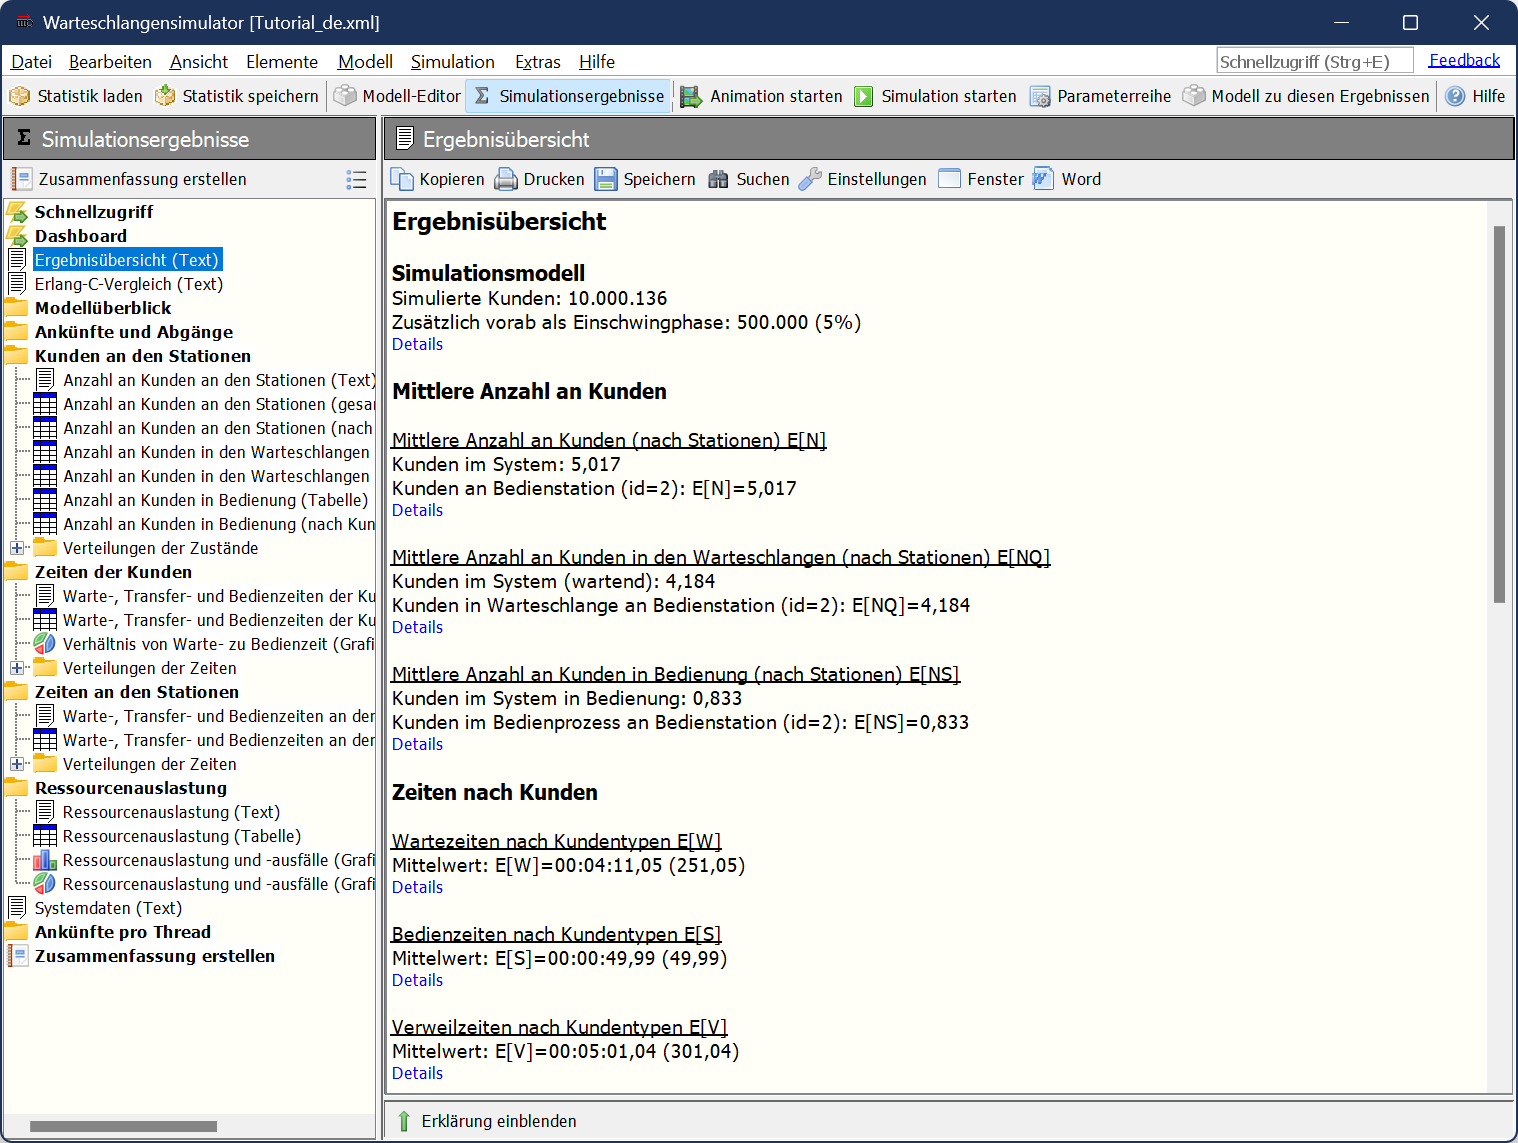
\includegraphics[width=14cm]{ProgramWindowResults.png}}
	\label{fig:ProgramWindowResults}
\end{figure} 

Die Simulationsergebnisse-Seite besteht auf der linken Seite aus einer Baumstruktur, in der die gewünschten Daten ausgewählt werden können, und auf der rechten Seite aus einem Anzeigebereich für die jeweils gewählte Information. Standardmäßig wird zunächst die ,,Ergebnisübersicht''-Seite dargestellt, auf der die am häufigsten benötigten Informationen dargestellt werden. Hier werden die mittleren Anzahlen an Kunden im System und an den Warteschlangen sowie die mittleren Warte- und Bediendauern und auch die Auslastungen der Bedienergruppen dargestellt.

Über die Schaltflächen ,,Kopieren'', ,,Drucken'' und ,,Speichern'' über der jeweiligen Ergebnisansicht können die Daten exportiert werden. Zum Speichern stehen dabei jeweils in Abhängigkeit von der dargestellten Information (Text, Tabelle, Grafik) verschiedene Formate inkl. Word-Dokumenten, Excel-Tabellen und pdf-Dateien zur Verfügung.

Von besonderer Bedeutung sind der erste und der letzte Eintrag in der Baumstruktur auf der linken Fensterseite: Der \textbf{Schnellzugriff} (erster Eintrag in der Baumstruktur) ermöglicht es, über einfache Javascript-Befehle eigene Ausgabeformate zu definieren. Auf diese Weise kann, wenn eine ganze Reihe von Modellen nacheinander simuliert werden sollen, stets auf die Informationen in der Darstellungsweise zugegriffen werden, die für die jeweilige Dokumentation der Ergebnisse notwendig sind. Über den Eintrag \textbf{Zusammenfassung erstellen} ganz unten in der Baumstruktur können Reports, die mehrere Einzeldokumente enthalten, erstellt werden. Als Ausgabeformate stehen hier docx-, pdf- und html-Dateien zur Verfügung. Des Weiteren können alle Tabelleninformationen, die in der Baumstruktur abrufbar sind, als Arbeitsblätter gesammelt in einer Excel-Arbeitsmappe gespeichert werden.

In der oberen Symbolleiste wird, wenn die Simulationsergebnis-Ansicht aktiv ist, der Eintrag \textbf{Modell zu diesen Ergebnissen} angezeigt. Über diese Schaltfläche kann jederzeit das Modell, das den Simulationsergebnissen zugrunde liegt, angezeigt werden. Die Idee ist hier folgende: Werden die Ergebnisse einer Simulation gespeichert, so wird in der Statistikdatei auch das vollständige Modell gespeichert. Auf diese Weise kann später, wenn die Statistikergebnisse wieder in den Simulator geladen wurden, stets nachvollzogen werden, auf welches Modell sich die Ergebnisse beziehen, d.\,h.\ eine separate Dokumentation von Modellen und Ergebnissen ist nicht notwendig. Die Simulationsergebnisse enthalten stets die Modelle. Wird auf die ,,Modell zu diesen Ergebnissen''-Schaltfläche geklickt, so öffnet sich ein Modell-Editor im Nur-Lese-Modus in einem neuen Fenster. So kann das Modell direkt betrachtet werden. Soll das Modell als Basis für weitere Simulationen verwendet werden, so kann es aus diesem Modell-Ansicht-Fenster über die \textbf{Modell in Editor laden} Schaltfläche auch jederzeit wieder in den normalen Modell-Editor geladen werden.



\chapter{Animation}

Die Animationsfunktion, die genauso wie die Simulationsfunktion über den entsprechenden Eintrag in der horizontalen Symbolleiste (,,\textbf{Animation starten}'') oder über die F6-Taste gestartet werden kann, dient der Visualisierung der Abläufe im Simulationsmodell.

Der Simulationskern des Warteschlangensimulators ist primär auf die klassische Simulation zur Generierung von statistischen Daten und nicht unmittelbar auf die Animation ausgelegt. Bei der ereignisorientierten stochastischen Simulation werden Ereignisse sequenziell abgearbeitet; im Simulationsablauf existieren nur die Zeitpunkte, an denen ein Ereignis auftritt. Von daher müssen Anpassungen vorgenommen werden, um einen kontinuierlichen Ablauf der Simulation während der Animation zu simulieren. Die Animation wird z.\,B.\ künstlich verlangsamt, wenn zwischen zwei Ereignissen ein längerer zeitlicher Abstand existiert. Um jedoch eine flüssige Animation darzustellen, erfolgt diese Abbildung der Modellzeit auf die reale Zeit nicht linear. Aufgrund der sequenziellen Abarbeitung der Ereignisse kann es außerdem passieren, dass die Bewegung von zwei Kunden, die sich eigentlich zeitlich bewegen, nacheinander dargestellt wird.

\section{Spezielle Elemente für die Animation}

In der Elementen-Vorlagen-Leiste existiert die Rubrik ,,Animation'', die einige spezielle Elemente zur Visualisierung von bestimmten Eigenschaften beinhaltet. Während einer normalen Simulation besitzen diese Elemente keine Bedeutung. Nur im Animationsmodus werden die speziellen Eigenschaften sichtbar. Die Animationselemente erlauben es, bestimmte Parameter (z.\,B.\ aktuelle Auslastungen, Wartezeiten der Kunden usw.) als Zahlenwerte, Balken, Diagramme oder auch in Form einer Ampel darzustellen.

Die jeweils darzustellenden Werte werden dabei in Form von Formeln definiert. Der Zugriff auf Daten bestimmter Stationen erfolgt jeweils über deren ID, so liefert ,,WIP(2)'' die aktuelle Anzahl an Kunden (Work units in process) an der Station mit der ID 2. Kunden werden über die Station, an denen Sie generiert wurden, identifiziert. So liefert ,,Wartezeit\_avg(1)'' die mittlere Wartezeit der Kunden des Typs, die an der Kundenquelle mit der ID 1 generiert wurden. Die Berechnung erfolgt dabei auf Kundentyp-Basis und die Nennung der Station ist nur exemplarisch, d.\,h.\ existieren zwei Kundenquellen, die Kunden desselben Typs generieren, so wird über den obigen Befehl die mittlere Wartezeit über die Kunden der beiden Kundenquellen ausgegeben.
 
\begin{figure}[H]	
	\caption{,,Ausdruck bearbeiten''-Dialog}
	\centerline{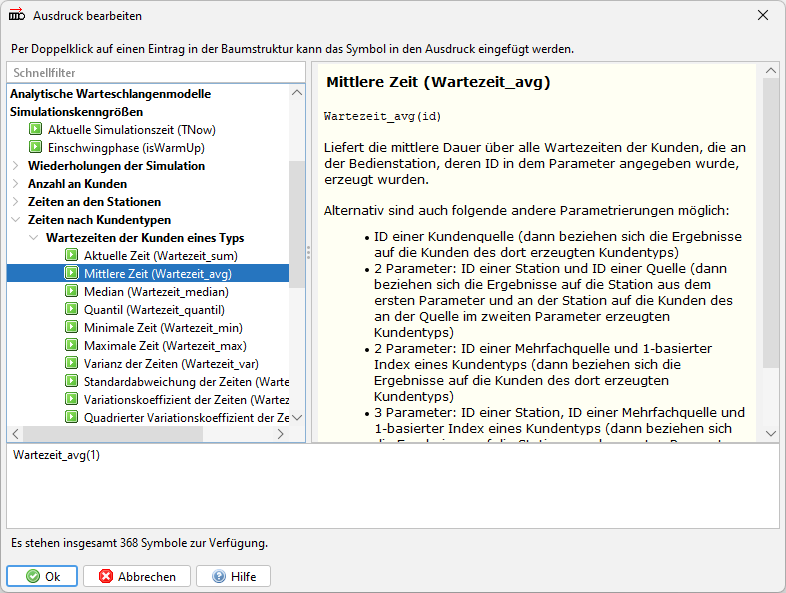
\includegraphics[width=14cm]{DialogExpressionBuilder.png}}
	\label{fig:DialogExpressionBuilder}
\end{figure} 

Eine Auflistung aller verfügbaren Befehle ist jeweils über der ,,Ausdruck bearbeiten''-Dialog abrufbar, der über das \textbf{Zauberstab-Symbol} rechts neben dem jeweiligen Formel-Eingabe-Feld abrufbar ist.

\section{Aufzeichnung von Animationen}

Über den Menüpunkt \textbf{Simulation|Animation aufzeichnen} ist es möglich, die Animation als avi-Videodatei aufzuzeichnen. Da der Warteschlangensimulator für die Aufzeichnung den mjpeg-Codec verwendet, in dem Einzelbilder gespeichert werden (im Gegensatz zu den für echte Videos verbreiteten Codecs mit Key-Frames und Zwischenbildern), fallen die Videodateien verhältnismäßig groß aus.



\chapter{Modelleigenschaften}

Ist der Modell-Editor aktiv, so kann über die Schaltfläche ,,Modell'' in der vertikalen Symbolleiste auf der linken Seite des Programmfensters der Modelleigenschaften-Dialog aufgerufen werden.
 
\begin{figure}[H]	
	\caption{,,Modelleigenschaften''-Dialog}
	\centerline{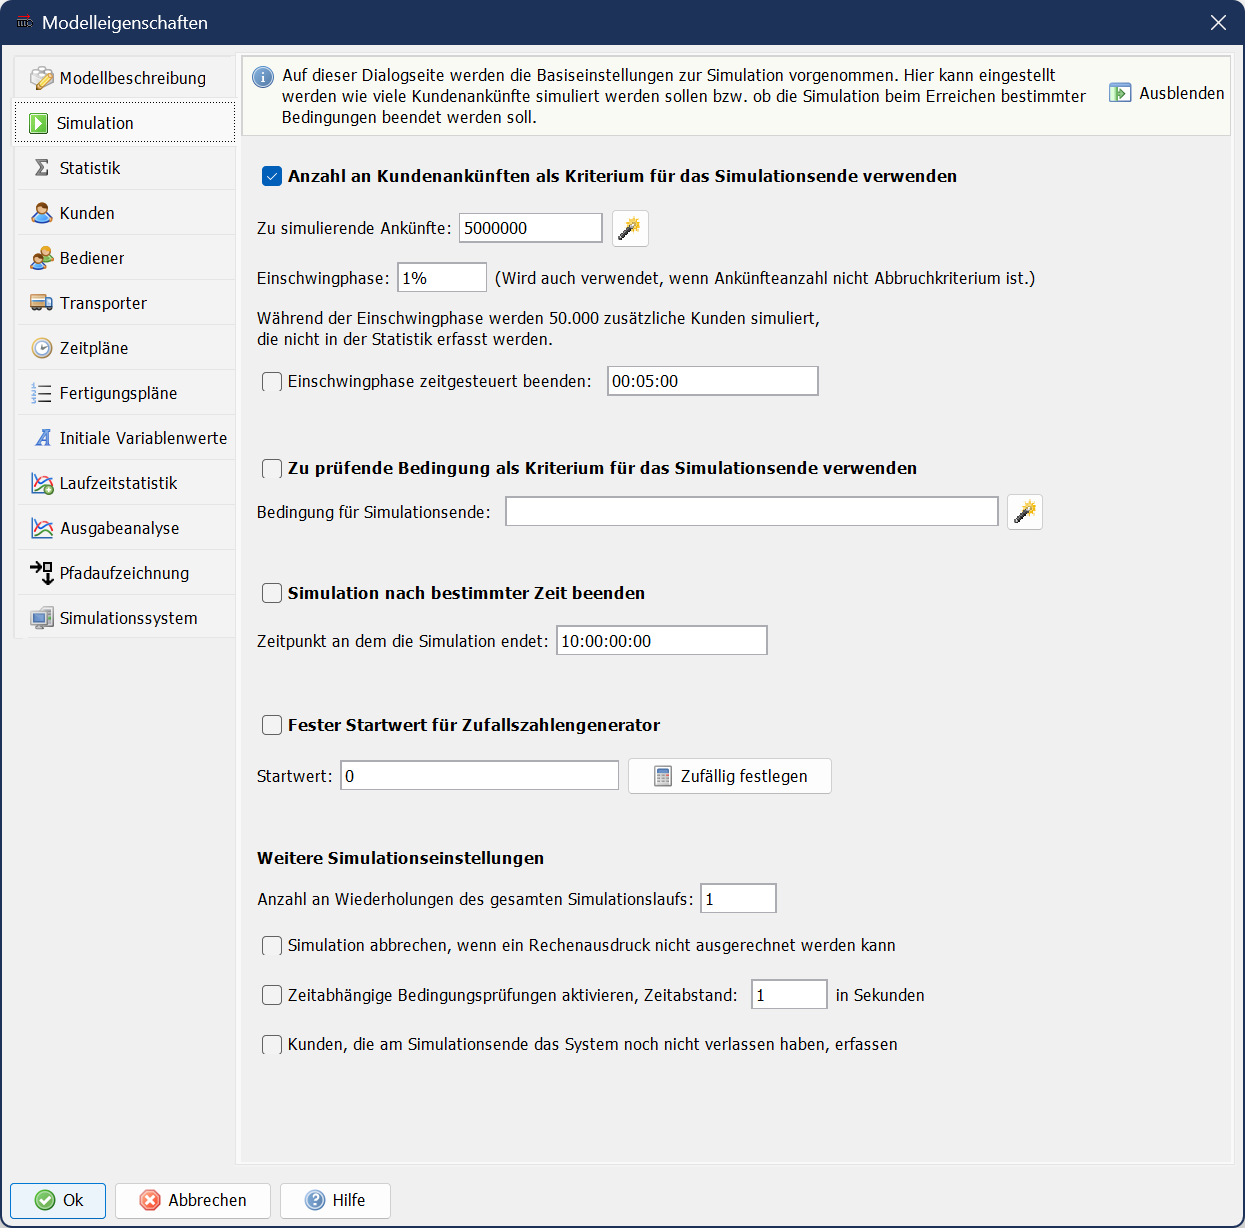
\includegraphics[width=14cm]{DialogModel.png}}
	\label{fig:DialogModel}
\end{figure} 

Dieser Dialog umfasst mehrere Registerreiter:

\begin{itemize}
\item
\textbf{Modellbeschreibung:}\\
Auf dieser Seite kann eine Beschreibung des Modells eingetragen werden. Diese Beschreibung hat keine Bedeutung für die Simulation, wird aber zusammen mit dem Simulationsmodell gespeichert und kann so zum späteren Wiederauffinden des Modells bzw. um später die Bedeutung des Modells nachvollziehen zu können, verwendet werden.
\item
\textbf{Simulation:}\\
Auf dieser Dialogseite kann eingestellt werden, wie lange und wie viele Male das Modell simuliert werden soll. Standardmäßig wird das Modell einmal simuliert und die Simulation wird beendet, wenn eine bestimmte Anzahl an Kunden das System durchlaufen hat (als Vorgabewert sind 10.000.000 eingestellt). Alternativ kann auch eine Abbruchbedingung, die während der Simulation fortwährend geprüft wird, oder aber ein Abbruchzeitpunkt (gemessen in der Zeit in der Simulation) angegeben werden.

Des Weiteren kann auf dieser Seite eingestellt werden, wie lange die Warm-up-Phase (oder auch Einschwing-Phase genannt) dauern soll. Eine Warm-Up-Phase von 1\% bei insgesamt 5.000.000 simulierten Kunden bedeutet, dass in Summe 5.050.000 (=5.000.000 $\cdot$ 101\%) Kunden simuliert werden. Die Erfassung der Statistikergebnisse beginnt jedoch erst ab dem 50.001ten Kunden. Auf diese Weise können Randeffekt in der Simulation ausgeblendet werden.

Auch kann optional ein fester Startwert für die Erzeugung von Zufallszahlen eingetragen werden. Dies ist insbesondere für die Animation von Modellen interessant. Ist die Funktion zur Verwendung eines festen Startwertes aktiv, so wird bei jedem Start von Simulation oder Animation exakt dieselbe Folge an Pseudozufallszahlen verwendet. Auf diese Weise lassen sich exakt reproduzierbare Ergebnisse erzielen. Da die Verwendung eines festen Startwertes für die Zufallszahlenerzeugung den Simulator jedoch daran hindert, die Simulation über mehrere CPU-Kerne zu parallelisieren, sollte diese nur aktiviert werden, wenn der Effekt der exakt selben Pseudozufallszahlen wirklich benötigt wird.
\item
\textbf{Kunden:}\\
Auf der Kunden-Dialogseite des Modeleigenschaften-Dialogs werden automatisch alle Kundentypen, die in dem Modell auftreten, aufgelistet. Pro Kundentyp können zum einen Eigenschaften, die für die Animation (Aussehen des Icons, das den Kunden repräsentiert) und die Statistik (Farbe der Balken für den jeweiligen Kundentyp in der Statistik) von Bedeutung sind, eingestellt werden und zum anderen können Kosten, die pro Warte-, Transfer- und Bediensekunde für Kunden des jeweiligen Typs anfallen, festgelegt werden.
\item
\textbf{Bediener:}\\
Auf dieser Seite werden die in dem Modell vorhandenen Bedienergruppen definiert. Praktisch kann es sich bei den ,,Bedienern'' um beliebige, für den Ablauf notwendige Ressourcen handeln, also z.\,B.\ auch um bestimmte Werkzeuge, die im Fabrikationsprozess benötigt werden usw. Beim Konfigurieren einer Bedienstation wird häufig direkt eine Bedienergruppe angelegt. In dem Einstellungen-Dialog der Bedienstation kann jedoch nur der Name der neuen Bedienergruppe festgelegt werden. Im Modelleinstellungen-Dialog kann festgelegt werden, wie viele Bediener in den jeweiligen Gruppen vorhanden sein sollen (neben einer festen Anzahl ist hier auch die Option ,,unendlich viele'' oder die Angabe eines Schichtplans möglich) und welche Kosten pro Verfügbarkeitsstunde, pro gearbeiteter Stunde und pro Leerlaufstunde anfallen sollen. Die Unterscheidung zwischen Verfügbarkeitsstunde und gearbeiteter Stunde ist insbesondere für Maschinen, die z.\,B.\ Strom verbrauchen, von Interesse: Über die Verfügbarkeitsstunden können z.\,B.\ Mietkosten für die Maschine, die pro Stunde anfallen, abgebildet werden. Die Kosten für die gearbeitete Zeit spiegeln dann die darauf aufzuschlagenden Stromkosten wider. Des Weiteren können Ausfall- bzw. Pausenzeiten für die Ressourcen definiert werden: Ein Bediener kann nach einer bestimmten Anzahl an Bedienungen, nach einer bestimmten Anwesenheitszeit oder nach einer bestimmten aktiv gearbeiteten Zeit in eine Pause gehen.
\item
\textbf{Transporter:}\\
Transporter können eingesetzt werden, um Kunden von Haltestellen zu Transportziel-Stationen zu transportieren. Transporter verhalten sich dabei ähnlich wie Ressourcen. Allerdings besitzen Transporter im Gegensatz zu Ressourcen einen definierten Aufenthaltsort. Dies bedeutet, dass die Transportzeit nicht über eine Verteilung definiert werden muss, sondern sich aus der Entfernung der Start- zur Zielstation ergibt. (Die Entfernungsmatrix zwischen den jeweiligen Stationen kann pro Transportertyp definiert werden.) Zusätzlich können pro Transportergruppe Lade- und Entladezeilen
definiert werden, die auf die Transportzeit aufaddiert werden, wenn Kunden transportiert wurden.
\item
\textbf{Zeitpläne:}\\
Zeitpläne können eingesetzt werden, um Zwischenankunftszeiten zwischen den Kunden an den Quelle-Stationen sowie die Verfügbarkeiten von Bedienern zu beschreiben. Als Basis für einen Zeitabschnitt innerhalb eines Zeitplans stehen die Werte eine Minute, 15 Minuten, 30 Minuten, eine Stunde und ein Tag zur Verfügung. Für jeden Zeitabschnitt kann ein individueller Wert eingestellt werden, der angibt, wie viele Kunden in diesem Zeitabschnitt eintreffen soll bzw. wie viele Bediener des jeweiligen Typs in dem Zeitabschnitt zur Verfügung stehen sollen. Zeitpläne können dabei beliebig lang sein. Zusätzlich kann eingestellt werden, wie am Ende des definierten Zeitplans verfahren werden soll: Der Zeitplan kann mit Nullen fortgesetzt werden, kann auf dem letzten Wert verharren, kann von Vorne wiederholt werden oder aber kann zunächst mit Nullen bis zum Ende des aktuellen Tages fortgesetzt werden und dann von neuem gestartet werden.
\item
\textbf{Fertigungspläne:}\\
Fertigungspläne werden in Kombination mit Transport-Elementen verwendet. Es gibt zwei Möglichkeiten zum Transport von Kunden zwischen Transport-Start- und Transport-Ziel-Elementen: Entweder ist direkt im Transport-Start-Element festgelegt, zu welchem Ziel Kunden welchen Typs transportiert werden sollen, oder aber die Information, welcher Kunde zu welchem Ziel geroutet werden möchte, wird mittels einem dem Kunden zugewiesenen Fertigungsplan direkt beim Kunden hinterlegt.
\item
\textbf{Initiale Variablenwerte:}\\
Variablen, die im Simulationsprozess verwendet werden, können auf dieser Dialogseite mit Initialwerten, die sofort von Beginn der Simulation an gelten, belegt werden. Auf diese Weise können z.\,B.\ Konstanten definiert werden, die an verschiedenen Stellen in Rechenausdrücken verwendet werden.
\item
\textbf{Laufzeitstatistik:}\\
Über diese Funktion können Ausdrücke, deren Wert sich über die Simulationszeit verändert und deren jeweils aktueller Wert für die Statistik erfasst werden soll, festgelegt werden.
\item
\textbf{Ausgabeanalyse:}\\
Der Simulator bietet zwei Funktionen zur Analyse der Simulationsergebnisse an: Zum einen kann eingestellt werden, dass während der Simulation die Autokorrelation der Wartezeiten ermittelt werden soll (d.\,h.\ wie häufig z.\,B.\ ein eine lange Wartezeit zur Folge, dass die nächsten Wartezeiten ebenfalls lang ausfallen). Diese Funktion ist im Normalfall ausgeschaltet, da sie die Simulation stark verlangsamt. Zum anderen kann eingestellt werden, ob basierend auf vorab (per Autokorrelations-Analyse) ermittelten Batch-Größen Konfidenzintervalle für verschiedene Kenngrößen berechnet werden sollen.
\item
\textbf{Pfadaufzeichnung:}\\
Optional kann die Bewegung der Kunden durch das System in Form einer Zählung der eingeschlagenen Pfade oder in Form der Zählung von Stationsübergängen erfasst werden.
Diese Zählung verlangsamt die Simulation und ist daher im Vorgabefall deaktiviert. Wird die Zählung aktiviert, so werden die erfassten Informationen über zusätzliche
Statistikseiten zum Abruf angeboten und auf ihrer Basis können auch Sankey-Diagramme, die die Bewegung der Kundenströme durch das System darstellen, erstellt werden.
\item
\textbf{Simulationssystem:}\\
Auf dieser Dialogseite können keine Einstellungen vorgenommen werden. Hier wird lediglich angezeigt, ob das Modell in seiner jetzigen Form in Ordnung ist bzw. an welcher Stelle ein Fehler vorliegt und ob das Modell über alle CPU-Kerne parallel simuliert werden kann und wenn nein, welche Eigenschaft dies verhindert.
\end{itemize}

\chapter{Weitere Elemente}

Neben den bisher vorgestellten Elementen zur Erzeugung (Quelle), Bedienung (Bedienstation) und zur Ausleitung der Kunden aus dem System (Ausgang) existieren noch eine Vielzahl weiterer Elemente in der Vorlagenleiste, die zum Ausbau von Modellen verwendet werden können. Die verfügbaren Elemente werden dabei thematisch gruppiert angeboten:

\begin{itemize}
\item
\textbf{Eingang/Ausgang:}\\
Enthält Elemente, über die neue Kunden in das System gelangen und über die Kunden am Ende das System wieder verlassen.
\item
\textbf{Verarbeitung:}\\
Enthält die klassischen Elemente zur Bedienung von Kunden bzw. zur Verzögerung der Kunden auf ihrem Weg durch das System.
\item
\textbf{Zuweisungen:}\\
Ermöglicht es Kunden spezielle Eigenschaften (z.\,B.\ einen neuen Kundentyp) zuzuordnen, Variablen oder Zählerstände zu verändern oder zusätzlich anfallende Kosten zu erfassen.
\item
\textbf{Verzweigungen:}\\
Über die Elemente in dieser Rubrik ist es möglich, Kunden basieren auf ihren Eigenschaften in verschiedene Richtungen weiter zu leiten, oder aber auch, Kunden zu duplizieren.
\item
\textbf{Schranken:}\\
Schranken ermöglichen es, Kunden zu verzögern bis bestimmte Bedingungen erfüllt sind. Es stehen dabei sowohl Elemente, die Kunden basierend auf einem zu prüfenden Ausdruck verzögern (auf diese Weise lässt sich prinzipiell alles abbilden, allerdings müssen jeweils passende Ausdrücke definiert werden), als auch Elemente, die die Verfügbarkeit von Ressourcen prüfen als auch klassische Schranken, die auf die Auslösung von Signal-Elementen reagieren, zur Verfügung.
\item
\textbf{Kunden verbinden:}\\
An vielen Produktionsprozessen werden an bestimmten Stellen Teil-Produktionsprozesse zu einem Prozess vereint, z.\,B.\ die Station, an der die Motoren in die Karosserien eingebaut werden. Die Elemente in dieser Rubrik ermöglichen die Abbildung solcher Vorgänge. Es existieren Elemente, in die zwei Kundenankunftsströme einlaufen (z.\,B.\ ,,Motor'' und ,,leere Karosserie''), die beiden Kunden an dieser Station aufhören zu existieren und stattdessen ein neuer Kunde (,,Karosserie mit Motor'') erstellt und weitergeleitet wird. Aber es kann auch einfach eine feste Anzahl an (möglicherweise gleichartigen) Objekten, die über eine gemeinsame Linie an einer Station eintreffen zu einem Batch bzw. neuen Objekt zusammengefasst werden. Die Verbindung der Elemente kann dabei temporär (d.\,h.\ später wieder auflösbar) oder dauerhaft sein.
Für die einfache Batch-Bedienung an einer Bedienstation müssen die Kunden jedoch überhaupt nicht vorab verbunden werden. Die Batch-Bedienung von einzeln eintreffenden Kunden kann direkt in dem Bedienstation-Element definiert werden.
\item
\textbf{Transport:}\\
Über die Transport-Elemente können Kunden von einer Station zu einer anderen, die mit der Ausgangsstation nicht verbunden ist, transportiert werden. Für die notwendige Transportdauer kann jeweils eine Zeitdauer angegeben werden und es können verschiedene Transportziele, die nach dem jeweiligen Kundentyp oder aber auch über einen Ausdruck bestimmt werden, angegeben werden.
\item
\textbf{Daten Ein-/Ausgabe}:\\
Über die Eingabe-Element können Zahlen aus Dateien oder Datenbanken geladen und an einer Variable zugewiesen werden.
Über die Ausgabe-Element können jederzeit Log-Datei-Einträge im Simulationsablauf generiert und in Dateien oder Datenbanktabellen gespeichert werden.
\item
\textbf{Flusssteuerungslogik:}\\
Die Flusssteuerungslogik-Elemente ermöglichen es, eine Flusssteuerung (bestehend aus bedingten Verzweigungen und Schleifen)
zu implementieren, die mit klassischen Programmiersprachen vergleichbar ist.
\item
\textbf{Analoge Werte:}\\
Mit Hilfe der Elemente in diesem Abschnitt können sich kontinuierlich ändernde Werte in der ansonsten diskret
ablaufenden Simulation abgebildet werden.
\item
\textbf{Animation:}\\
Die in dieser Rubrik versammelten Elemente dienen alle zur Visualisierung bestimmter Kenngrößen während der Animation. Die Darstellung der Werte kann dabei in Form von Texten, Balken, Liniendiagrammen oder auch in Form einer Ampel erfolgen. Für die klassische Simulation besitzen diese Elemente keine weitere Bedeutung.
\item
\textbf{Optische Gestaltung:}\\
Die Elemente in dieser Rubrik besitzen durchweg keine Bedeutung für die Simulation oder die Animation. Die Elemente dienen ausschließlich der optischen Gestaltung von Simulationsmodellen (z.\,B.\ zur Darstellung von Informationstexten oder zur Hervorhebung bestimmter Abschnitte durch farbige Kästen).
\item
\textbf{Sonstiges:}\\
In dieser Rubrik befinden sich ein ganz besonderes Elemente: Das Untermodell-Element ermöglicht es, vollständige Teilmodelle in eine einzelne Station zu verpacken, um so das Hauptmodell übersichtlicher zu halten.
\end{itemize}

\section{Beschreibung einiger dieser Elemente}

Die vollständige Beschreibung aller dieser Elemente würde den Rahmen dieser Einführung sprengen, daher sollen nur exemplarisch einige wenige Elemente vorgestellt werden:

\subsection*{Verzögerung-Element}

\begin{wrapfigure}{l}{2.25cm}
\vspace{-22pt}
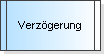
\includegraphics[width=2cm]{IconDelay.png}
\vspace{-22pt}
\end{wrapfigure}
Das Verzögerung-Element stellt eine einfachere Variante einer Bedienstation dar: Es gibt hier keine Warteschlange, sondern alle eintreffenden Kunden werden sofort bedient. Allerdings sind hierfür auch keine Bediener notwendig, sondern die Kunden werden einfach nur eine bestimmte, über eine Wahrscheinlichkeitsverteilung oder einen Ausdruck vorgebbare Zeitdauer verzögert. Es kann wieder eingestellt werden, ob die Verzögerung als Bedienzeit, als Transferzeit oder als Wartezeit in der Statistik erfasst werden soll.

\subsection*{Typzuweisung-Element}

\begin{wrapfigure}{l}{2.25cm}
\vspace{-22pt}
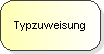
\includegraphics[width=2cm]{IconAssign.png}
\vspace{-22pt}
\end{wrapfigure}
Über das Typzuweisung-Element kann der Typ eines Kunden (unter dem später seine Daten in der Statistik erfasst werden), nachträglich verändert werden. Jeder Kunde erhält bereits durch die Kundenquelle einen bestimmten Typ. Sollen verschiedene Steuerungsalternativen verglichen werden, so kann es aus Vergleichbarkeitsgründen sinnvoll sein, diese mit exakt demselben Kundenankunftsstrom zu versorgen. Dies setzt man um, in dem der Kundenankunftsstrom nach der Erzeugung über ein Duplizieren-Element verdoppelt wird. Im Folgenden kann dann über ein Typzuweisung-Element jedem der beiden Teilströme ein individueller Kundentyp zugewiesen werden.

\vfill
\pagebreak

\subsection*{Verzweigen-Element}

\begin{wrapfigure}{l}{2.25cm}
\vspace{-22pt}
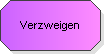
\includegraphics[width=2cm]{IconDecide.png}
\vspace{-22pt}
\end{wrapfigure}
Im Gegensatz zu den meisten Elementen, die zwar beliebig viele Ankunftskanten aufnehmen können, aber nur einen Ausgang besitzen, können beliebig viele Kanten aus dem Verzweigen-Element hinausführen. Über den Einstellungen-Dialog des Verzweigen-Elements kann eingestellt werden, nach welchen Kriterien die Kunden in die verschiedenen Richtungen geleitet werden sollen. Zur Auswahl stehen hierbei folgende Optionen:
\begin{itemize}
\item
Die Kunden können \textbf{zufällig} in die verschiedenen Richtungen geleitet werden (wobei pro Richtung eine Rate, mit der die Weiterleitung in diese Richtung erfolgt, angegeben werden kann).
\item
Die Kunden können jeweils gemäß bestimmten zu prüfenden \textbf{Bedingungen} in die verschiedenen Richtungen geleitet werden (z.\,B.\ in die Richtung der Station, an der sich momentan am wenigsten Kunden befinden).
\item
Die Kunden können gemäß dem \textbf{Typ des Kunden} in die verschiedenen Richtungen verzweigt werden.
\item
Es können alle Richtungen \textbf{reihum} bedingt werden.
\item
Der Ausgang kann gemäß bestimmten Eigenschaften der Folgestationen (z.\,B.\ \textbf{kürzeste Warteschlange}) gewählt werden.
\end{itemize}

\subsection*{Duplizieren-Element}

\begin{wrapfigure}{l}{2.25cm}
\vspace{-22pt}
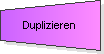
\includegraphics[width=2cm]{IconDuplicate.png}
\vspace{-22pt}
\end{wrapfigure}
Das Duplizieren Element besitzt ebenfalls mehrere Ausgangskanten. Im Gegensatz zu dem Verzweigen-Element wird ein eintreffender Kunde jedoch nicht über eine der Ausgangskanten weitergeleitet, sondern es werden Kopien der Kunden erstellt und es wird über jede der Kanten zeitgleich ein inhaltlich identisches Kundenobjekt weitergeleitet.

\subsection*{Bedingung-Element}

\begin{wrapfigure}{l}{2.25cm}
\vspace{-22pt}
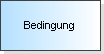
\includegraphics[width=2cm]{IconCondition.png}
\vspace{-22pt}
\end{wrapfigure}
An Bedingungen-Elementen können Kunden verzögert werden. Kunden werden nur so lange weitergeleitet, wie die angegebene Bedingung erfüllt ist. Z.\,B.\ kann über eine Bedingung-Element erfasst werden, wie viele Kunden sich in einem bestimmten Modellabschnitt befinden, nur wenn dieser Wert unter einem bestimmten Schwellenwert liegt, werden weitere Kunden in diesen Abschnitt geleitet.

\subsection*{Untermodell-Element}

\begin{wrapfigure}{l}{2.25cm}
\vspace{-22pt}
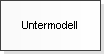
\includegraphics[width=2cm]{IconSubModel.png}
\vspace{-22pt}
\end{wrapfigure}
In ein Untermodell kann ein vollständiges Teil-Fließbild implementiert werden. Auf diese Weise können größere Modelle übersichtlicher gehalten werden. Nach außen sieht ein Untermodell-Element wie ein normales Element aus. In dem Eigenschaften-Dialog kann eingestellt werden, wie viele Eingangs- und Ausgangskanten es aufnehmen soll. Wird im Kontextmenü jedoch der Menüpunkt \textbf{Untermodell bearbeiten} angeklickt oder wird bei ausgewähltem Untermodell-Element die Tastenkombination Umschalt+Enter gedruckt, so öffnet sich ein weiterer Modell-Editor in einem Dialog. Die definierten Eingangs- und Ausgangskanten sind hier als nichtlöschbare Pseudo-Elemente dargestellt. Zwischen diesen kann das Untermodell erstellt werden.



\end{document}